\documentclass[11pt,letterpaper]{article}
\usepackage[margin=0.85in]{geometry}
\usepackage[T1]{fontenc}
\usepackage{lmodern,amsmath,amssymb,booktabs,graphicx,xcolor,fancyhdr}
\usepackage[colorlinks=true,linkcolor=blue!45!black,urlcolor=blue!45!black,citecolor=blue!45!black]{hyperref}
\setlength{\parindent}{0pt}
\setlength{\parskip}{6pt}
\setlength{\headheight}{14pt}
\pagestyle{fancy}\fancyhf{}
\fancyhead[L]{\small Alex Blythe / Aero}
\fancyhead[R]{\small Scalar transport, version 1.0}
\fancyfoot[L]{\small Numerical verification; no experimental validation}
\fancyfoot[R]{\small\thepage}
\newcommand{\note}[1]{\begin{quote}\small\textbf{Scope.} #1\end{quote}}
\begin{document}
\begin{center}
{\LARGE\bfseries Square-body scalar transport}\par\vspace{5pt}
{\large A functional spreadsheet and browser model:\par accuracy, assumptions, and worked examples}\par\vspace{8pt}
Alex Blythe \quad 24 October 2026 \quad Version 1.0
\end{center}
\note{This model solves a scalar equation in a prescribed horizontal velocity field. It does not solve fluid velocity, pressure, drag, or vortex shedding. Close agreement between implementations establishes agreement on the stated discrete equations, not physical accuracy of flow around a solid.}

\section*{1. Problem and reconstruction}
The model reconstructs the transport calculation visible in user-supplied screenshots from \href{https://www.instagram.com/cfdbyhand/}{@cfdbyhand}. The original workbook and narration were unavailable. This is an independently authored implementation, with attribution for teaching inspiration rather than a claim of affiliation or exact reproduction.

The transported scalar $\phi$ is dimensionless. For constant prescribed $u\geq0$, density $\rho$, and transport coefficient $\Gamma$, the modeled equation is
\begin{equation}
\rho u\frac{\partial\phi}{\partial x}
=\Gamma\left(\frac{\partial^2\phi}{\partial x^2}+\frac{\partial^2\phi}{\partial y^2}\right).
\label{eq:pde}
\end{equation}
The rectangle is $0\leq x\leq L$, $0\leq y\leq H$. The square is a region where grid-node scalar values are held at $\phi_s$. It is not an impermeable, no-slip obstacle in a solved velocity field. The prescribed velocity remains unchanged.

\begin{center}\small
\begin{tabular}{lll}
\toprule Quantity & Baseline value & Provenance \\\midrule
$u,\rho,\Gamma$ & $1\ \mathrm{m/s},\ 1\ \mathrm{kg/m^3},\ 0.1\ \mathrm{kg/(m\,s)}$ & Visible screenshot inputs \\
$\Delta x,\Delta y$ & $0.05\ \mathrm{m}$ each & Visible screenshot spacing \\
$L,H$ & $3\ \mathrm{m},\ 2\ \mathrm{m}$ & Reconstruction assumptions \\
Square corner and side & $(0.8,0.75)\ \mathrm{m}$; $0.5\ \mathrm{m}$ & Reconstruction assumptions \\
$\phi_{\rm in},\phi_s$ & $1,0$ & Reconstructed boundary setup \\
Grid & $61\times41$ nodes & Derived from domain and spacing \\
\bottomrule
\end{tabular}
\end{center}

The left boundary holds $\phi=\phi_{\rm in}$. The right boundary copies its left neighbor, approximating $\partial\phi/\partial x=0$. Top and bottom copy the adjacent interior row, approximating $\partial\phi/\partial y=0$. Boundary copying is first-order. Inlet conditions take precedence at the left corners. Square nodes, including their geometric boundary, are fixed. Geometry changes snap to included nodes with a $10^{-9}$ m comparison allowance.

The rectangle's transverse boundaries represent zero scalar gradient. They are not evidence that a hydrodynamic symmetry condition has been satisfied. Background discretization references are provided by NIST FiPy \cite{nistdiscrete,nistscheme}.

\newpage
\section*{2. Discretization and accuracy}
For an interior node and positive $u$, the model uses upwind advection and centered diffusion. In conductance notation,
\begin{align}
D_x&=\Gamma\frac{\Delta y}{\Delta x},&D_y&=\Gamma\frac{\Delta x}{\Delta y},&F&=\rho u\Delta y,\\
a_W&=D_x+F,&a_E&=D_x,&a_N=a_S&=D_y,\\
\phi_P&=\frac{a_W\phi_W+a_E\phi_E+a_N\phi_N+a_S\phi_S}{a_P},&&a_P=a_W+a_E+a_N+a_S.
\end{align}
At baseline, $D_x=D_y=0.1$, $F=0.05$, and $a_P=0.45$. The denominator is included. The cell P\'eclet number is $F/D_x=0.5$.

Upwind advection is first-order. A Taylor expansion of the backward derivative introduces leading streamwise numerical diffusion
\begin{equation}
\Gamma_{\rm num}\simeq \frac{\rho u\Delta x}{2}=0.025\ \mathrm{kg/(m\,s)}.
\end{equation}
This is 25\% of the specified baseline $\Gamma$. \textbf{It is a truncation-error coefficient ratio, not a 25\% solution-error claim.} Its derivation assumes a smooth solution away from boundaries and corners. NIST discusses the upwind scheme's excess numerical diffusion \cite{nistscheme}.

\textbf{Analytical check.} A separate one-dimensional problem uses $L=1$, $\rho=u=1$, $\Gamma=0.1$, $\phi(0)=0$, and $\phi(1)=1$. These Dirichlet conditions differ from the square example. Its exact solution is
\begin{equation}
\phi(x)=\frac{\exp(10x)-1}{\exp(10)-1}.
\end{equation}
\begin{center}
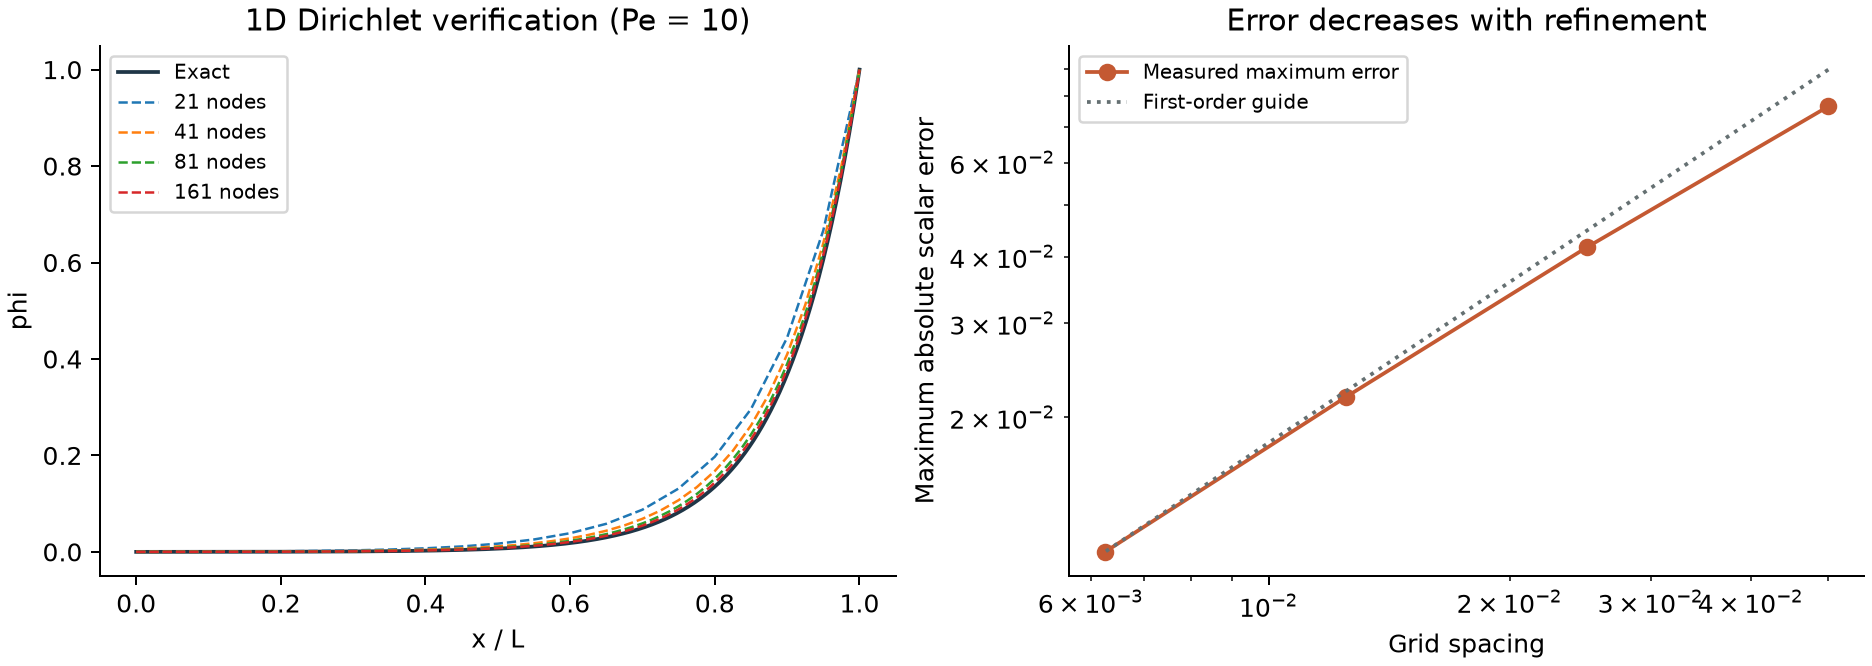
\includegraphics[width=\linewidth]{figures/analytical.png}
\end{center}
\begin{center}\small\begin{tabular}{rrrr}
\toprule
Nodes & $h$ & $\|e\|_\infty$ & Observed order \\
\midrule
21 & 0.05000 & 0.07643 & -- \\
41 & 0.02500 & 0.04167 & 0.875 \\
81 & 0.01250 & 0.02184 & 0.932 \\
161 & 0.00625 & 0.01120 & 0.964 \\
\bottomrule
\end{tabular}
\end{center}
The observed order approaches one. Error is absolute scalar error; dividing by near-zero exact values would give misleading relative errors. This test verifies the scheme, not an error bound for the square geometry.

\newpage
\section*{3. Worked examples}
All four examples use the baseline domain, density, transport coefficient, and grid. The square is shown as white because its scalar is prescribed, not because velocity has been solved around it. A fixed color scale permits comparisons.
\begin{center}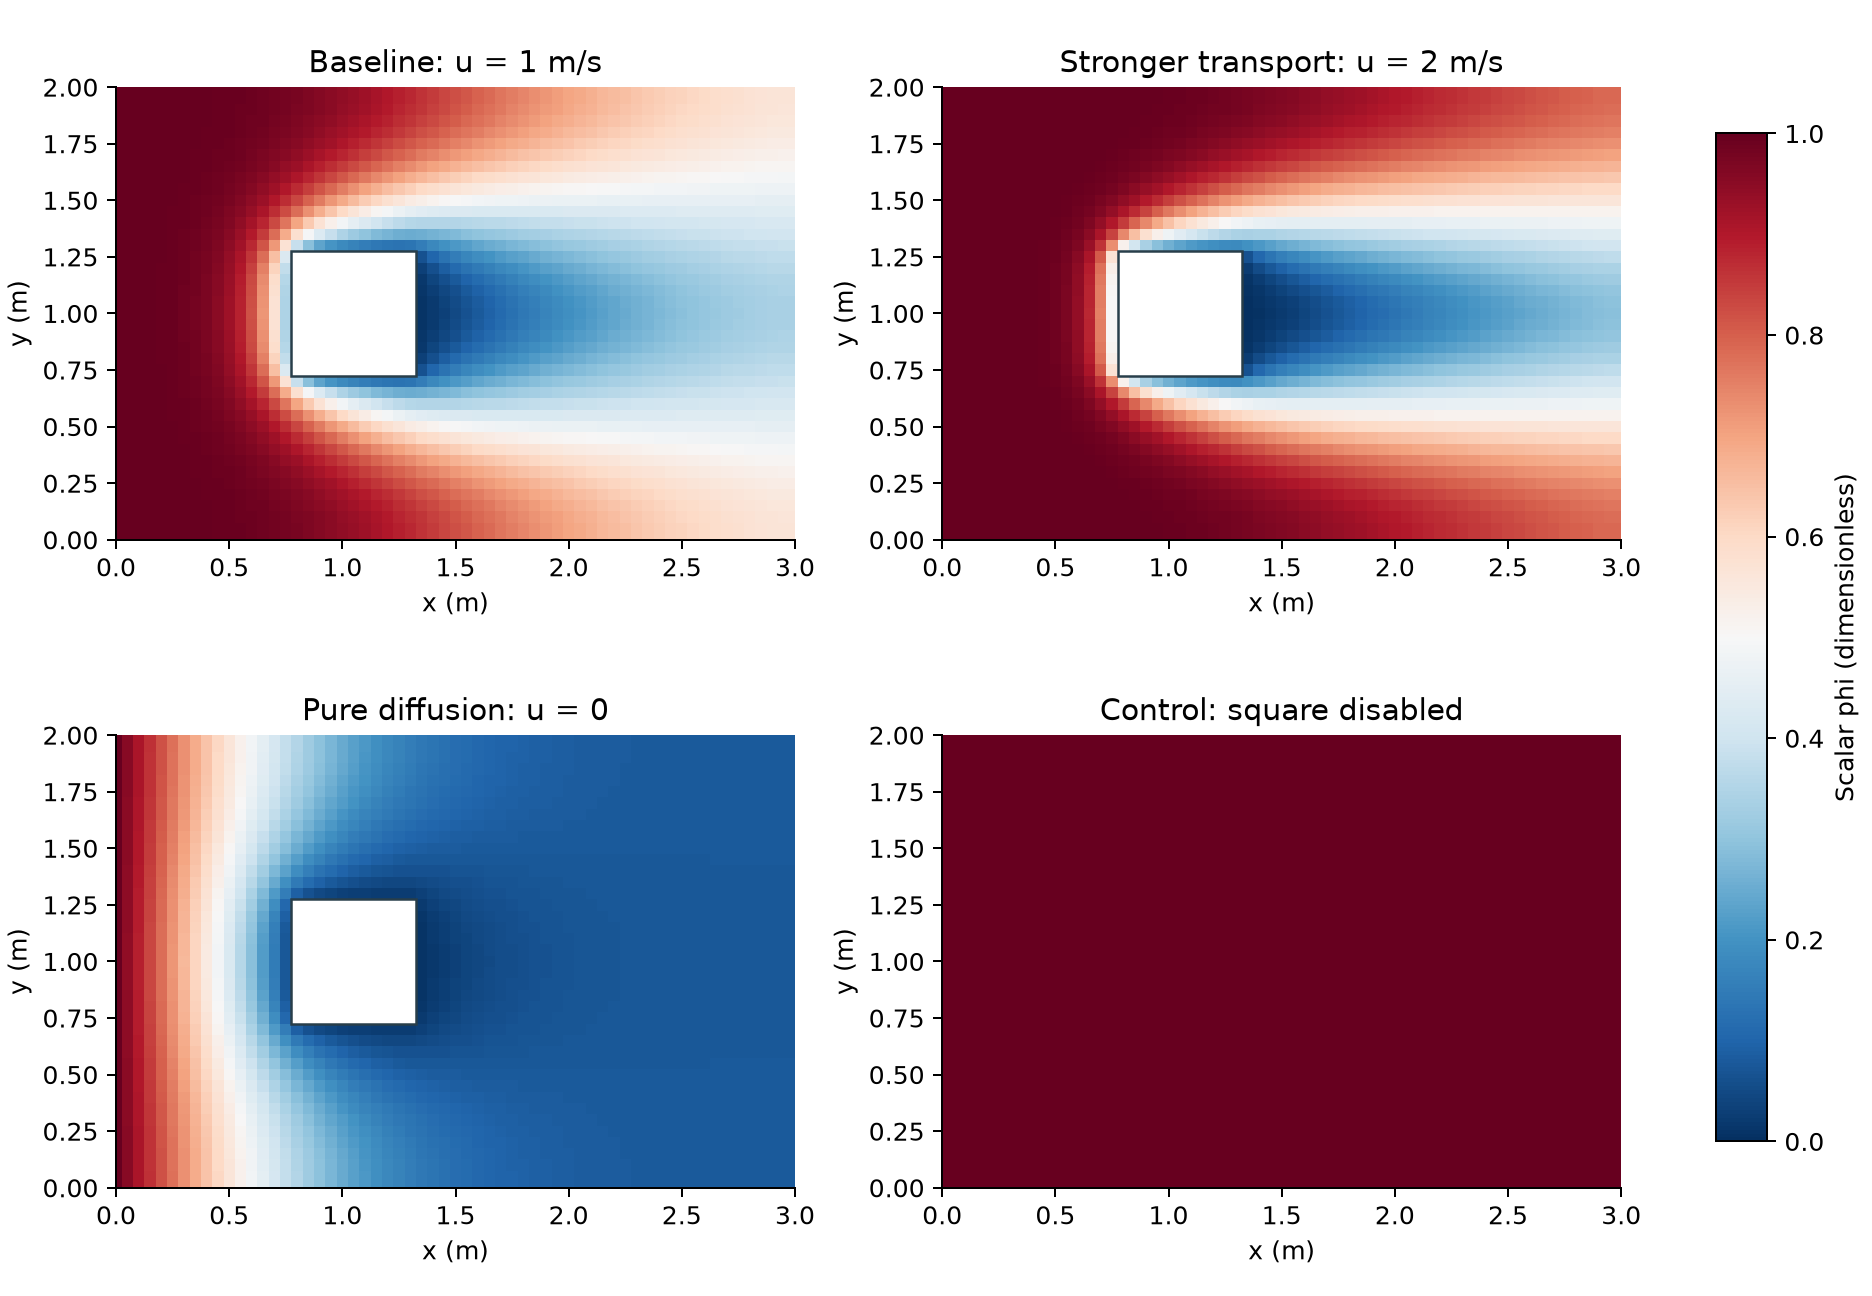
\includegraphics[width=\linewidth]{figures/examples.png}\end{center}
\begin{center}\small
\begin{tabular}{llrr}
\toprule Example & Change & $u$ (m/s) & $\phi(3,1)$ \\\midrule
Baseline & None & 1 & 0.338126 \\
Stronger transport & Double velocity & 2 & 0.290217 \\
Pure diffusion & Remove advection & 0 & 0.077516 \\
Uniform control & Disable square clamp & 1 & 1.000000 \\
\bottomrule\end{tabular}
\end{center}

\textbf{Interpretation.} Increasing transport speed changes the extent and recovery of the scalar deficit. Removing advection leaves a diffusion problem driven by the inlet and the square clamp. Disabling the square admits the exact uniform solution $\phi=1$, which checks the boundary setup and constant preservation.

These pictures do not show streamlines, pressure, momentum loss, or vorticity. The scalar deficit downstream is not an aerodynamic wake prediction. No physical interpretation such as concentration or normalized temperature is assigned without the additional constitutive and boundary assumptions that interpretation requires.

\newpage
\section*{4. Executed numerical evidence}
\textbf{Independent assembly and solution.} A Python implementation assembles the linear equations as a sparse matrix and uses SciPy \texttt{spsolve}. It does not call the JavaScript solver. GS below denotes the separate Gauss--Seidel reference. The normalized residual is
\begin{equation}
r_\infty=\max_P\left|\frac{(A\phi-b)_P}{A_{PP}}\right|,
\end{equation}
including boundary rows. This has scalar units and is equivalent to the maximum normalized stencil defect. It is not a continuum error estimate.
\begin{center}\small\begin{tabular}{lrr}
\toprule
Case & $\|\phi_{LU}-\phi_{GS}\|_\infty$ & LU residual \\
\midrule
baseline & 3.88e-11 & 4.93e-16 \\
faster & 1.38e-11 & 7.77e-16 \\
diffusion & 1.17e-09 & 4.51e-16 \\
uniform & 2.00e-14 & 6.78e-16 \\
\bottomrule
\end{tabular}
\end{center}
Four direct solutions also remain within the specified scalar bounds, allowing $10^{-10}$ roundoff. The largest LU-to-GS difference is $1.17\times10^{-9}$, in pure diffusion. Two implementations can share a modeling error; the analytical test addresses an additional, different question.

\textbf{Native workbook checks.} Microsoft Excel 16.0, build 20326 recalculated the workbook, changed velocity, disabled the square, selected pure diffusion, restored defaults, and saved/reopened the result. All 2,501 field formulas and the iteration settings were retained.
\begin{center}\small\begin{tabular}{lrr}
\toprule
Case & Excel vs. GS maximum difference & Excel residual \\
\midrule
baseline & 1.89e-12 & 9.33e-13 \\
faster & 1.33e-09 & 9.23e-11 \\
uniform & 4.10e-09 & 9.71e-11 \\
diffusion & 1.16e-07 & 9.99e-11 \\
\bottomrule
\end{tabular}
\end{center}
Excel uses at most 10,000 iterations per calculation with maximum change $10^{-10}$. A small change or residual is not an accuracy certificate. Pure diffusion may take substantially longer than the baseline. The browser worker's message path and invalid-input handling were exercised in a Node worker harness; this is not a claim of cross-browser UI validation.

\textbf{Square-case refinement.} Three aligned grids preserve the physical square coordinates and include its boundary nodes. Common-node changes compare adjacent grids at shared fluid nodes.
\begin{center}\small\begin{tabular}{lrrrr}
\toprule
Grid & $h_x$ (m) & $\phi(2,1)$ & $\phi(3,1)$ & Common-node change \\
\midrule
61 $\times$ 41 & 0.0500 & 0.194275 & 0.338126 & -- \\
121 $\times$ 81 & 0.0250 & 0.199701 & 0.348439 & 0.04701 \\
241 $\times$ 161 & 0.0125 & 0.202145 & 0.353281 & 0.02721 \\
\bottomrule
\end{tabular}
\end{center}
The outlet-center value changes by about 0.01516 between the first and finest grids. The maximum common-node differences remain 0.04701 and 0.02721. \textbf{The baseline is mesh-dependent.} The finest result is a comparison, not an exact solution. Corner behavior and first-order boundary treatment affect the trend. No formal error bound, grid-convergence index, or grid-independence claim is made.

\newpage
\section*{5. Use, reproduction, and limits}
\textbf{Workbook.} Open \texttt{Square\_Body\_Transport.xlsx} in desktop Excel and edit amber inputs on Model. Field contains the cell equations and residual. Allow iterative calculation and press F9 if necessary. The workbook settings are 10,000 iterations and maximum change $10^{-10}$. Other open workbooks can affect Excel calculation settings. No macros, external workbook links, or private service connections are required.

\textbf{Browser.} The worker solves the same nodal model locally. Geometry stays on the fixed grid. Input changes require a new calculation; any retained result is explicitly identified as the previous completed solve. Stop cancels the worker. A completed field can be downloaded as CSV. The UI reports iteration count, residual, cell P\'eclet number, and outlet-center scalar. A stalled iteration limit is reported as unconverged, not accepted.

\textbf{Reproduce.} The public package contains the browser solver and worker, independent verification script, versioned inputs, workbook reference fields, Excel verification summary, CSVs, accuracy measurements, and a SHA-256 manifest. In a new environment with Python, install \texttt{numpy scipy matplotlib}, then run:
\begin{quote}\small\ttfamily
python verify\_accuracy.py --output .
\end{quote}
Run this from an extracted reproduction package containing the supplied reference JSON files. The script rebuilds the sparse, analytical, and refinement checks and figures. It does not rerun Excel. The retained Excel measurements describe the recorded desktop run. Compile \texttt{main.tex} inside the LaTeX source directory with a normal LaTeX engine or Tectonic.

\textbf{Remaining limits.} The model is linear, steady, two-dimensional, and limited to nonnegative prescribed horizontal velocity with positive density and diffusion. The square prescribes scalar; it does not enforce no-penetration or no-slip in a solved velocity field. There is no turbulence, transition, compressibility, momentum coupling, pressure correction, or unsteady shedding model. Domain adequacy and experimental agreement are unestablished. The screenshot-derived values do not define a validated material or flow regime. The results are educational numerical evidence, not an aerodynamic design release.

\textbf{Next physical extension.} Introduce continuity and both momentum equations, a pressure projection or correction, no-slip/no-penetration boundaries, and appropriate unsteady treatment. Verify against independent reference quantities before reporting drag, separation, or wake dynamics. Those additions would change the model's governing problem rather than merely improve its color plot.

\begin{thebibliography}{9}\small
\bibitem{nistdiscrete} NIST FiPy, \emph{Finite Volume Method}. \url{https://pages.nist.gov/fipy/en/stable/numerical/discret.html}. Accessed 24 October 2026. Background reference; this implementation uses a nodal stencil, not FiPy itself.
\bibitem{nistscheme} NIST FiPy, \emph{Numerical Schemes}. \url{https://pages.nist.gov/fipy/en/3.4.5/numerical/scheme.html}. Accessed 24 October 2026.
\bibitem{inspiration} CFDbyHand, Instagram profile \texttt{@cfdbyhand}. \url{https://www.instagram.com/cfdbyhand/}. Teaching inspiration reviewed from user-supplied screenshots; original workbook not obtained.
\bibitem{evidence} Alex Blythe, \emph{Square-body scalar transport, version 1.0: executable evidence and downloads}. \url{https://alex-blythe.com/software/aero/square-body-transport/}. 24 October 2026. See \texttt{accuracy-results.json}, \texttt{excel-verification.json}, and \texttt{browser-solver-checks.json}.
\end{thebibliography}
\end{document}
